\subsection{Scale-Invariant Feature Transform (SIFT)}
David G. Lowe hat mit der Einführung des SIFT-Algorithmus einen für die
Bildverarbeitung wertvollen Beitrag geleistet. Der SIFT-Algoritmus findet lokale
Merkmale in Bildern. Diese Merkmale sind invariant gegenüber Bildskalierung und
-drehung und teilweise invariant gegenüber Änderungen der Beleuchtung sowie des
Betrachtungswinkels. Die Wahrscheinlichkeit einer Störung durch Verdeckung
einzelner Elemente oder auftretenden Bildrauschens wird, durch räumliche
Streuung und einem vielseitigen Frequenzbereich, erreicht. Im Folgenden wird die
grobe Vorgehensweise zur Findung der lokalen Merkmale erläutert.
\parencite{sift-distinctive-features}

\begin{enumerate}
    \item \textbf{Scale-space extrema detection}\newline
    Zu Beginn wird aus einem Bild durch repetetives Unschärfen (mittels
    \textit{Gaußschen Weichzeichner}\footnote{https://datacarpentry.org/image-processing/06-blurring/ [09.12.2022]})
    und Halbieren der Größe eine Serie an Bildern erzeugt (siehe Abbildung
    \ref{fig:sift1}). Auf die Bilder der Bilderserie folgt die Anwendung der
    \textit{Gaußschen Differenzfunktion}\footnote{https://www.sciencedirect.com/science/article/pii/B9780123694072500097 [09.12.2022]}
    (siehe Abbildung \ref{fig:sift2}). \parencite{sift-web-scale-space}

    \begin{figure}[H]
        \centering
        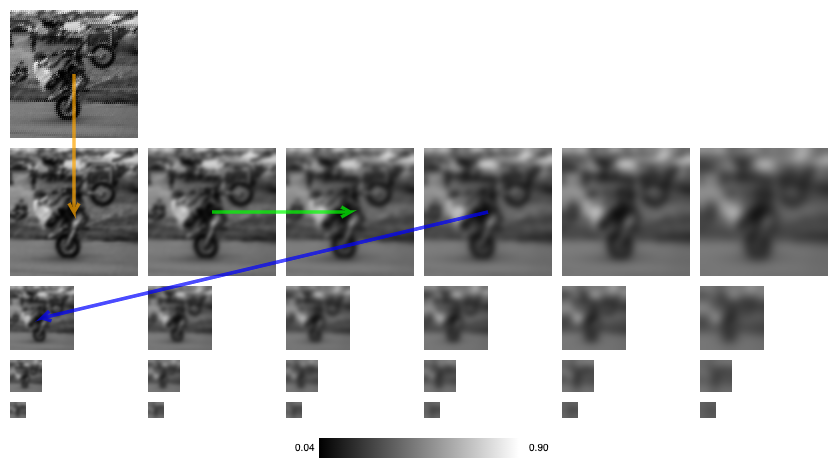
\includegraphics[width=13.3cm]{sift-1}
        \caption{SIFT: Erzeugung der Bilderserie}
        \label{fig:sift1}
        \bildquelle{Eigene Darstellung; http://weitz.de/sift/}
    \end{figure}

    \begin{figure}[H]
        \centering
        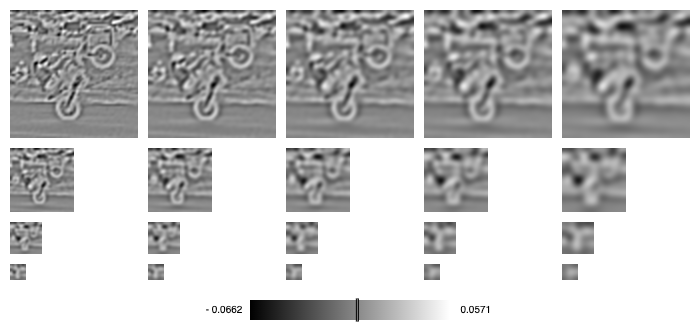
\includegraphics[width=13.3cm]{sift-2}
        \caption{SIFT: Anwendung Gaußscher Differenzfunktion}
        \label{fig:sift2}
        \bildquelle{Eigene Darstellung; http://weitz.de/sift/}
    \end{figure}

    \item \textbf{Keypoint localization}\newline
    Aus den vorher differenzierten Grafiken werden mit dem
    \textit{Marr-Hildreth-Operator}\footnote{https://theailearner.com/2019/05/25/laplacian-of-gaussian-log [09.12.2022]}
    interessante Schlüsselpunkte bzw. Merkmale herausgefiltert (siehe Abbildung
    \ref{fig:sift3}) \parencite{sift-web-keypoint}. Eine dem \textit{Harris-Corner-Detector}\footnote{https://docs.opencv.org/3.4/dc/d0d/tutorial\_py\_features\_harris.html [09.12.2022]}
    ähnliche Prozedur wird angewandt, um unwichtige Punkte herauszusieben
    (siehe Abbildung \ref{fig:sift5}) \parencite{sift-web-low-contrast}.

    \begin{figure}[H]
        \centering
        \begin{subfigure}{.5\textwidth}
          \centering
          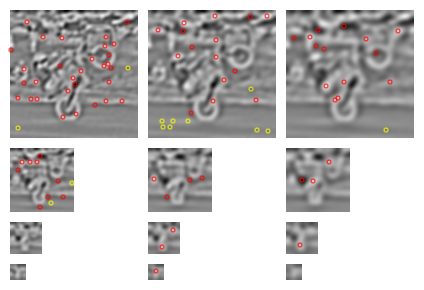
\includegraphics[width=.75\linewidth]{sift-3}
          \caption{Extrahierte Schlüsselpunkte}
          \label{fig:sift3}
        \end{subfigure}%
        \begin{subfigure}{.5\textwidth}
          \centering
          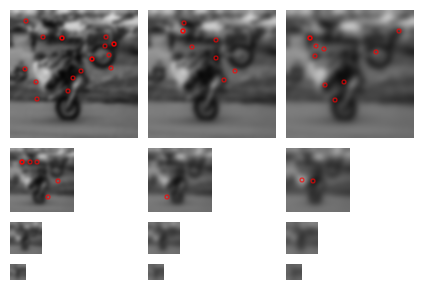
\includegraphics[width=.75\linewidth]{sift-5}
          \caption{Filterung unwichtiger Schlüsselpunkte}
          \label{fig:sift5}
        \end{subfigure}
        \caption{SIFT: Schlüsselpunkt-Lokalisierung}
        \label{fig:sift-keypoint}
        \bildquelle{Eigene Darstellung; http://weitz.de/sift/}
    \end{figure}

    \item \textbf{Orientation assignment}\newline
    Mithilfe eines Histogramms kann den Schlüsselpunkten nun eine Orientierung
    zugewiesen werden (siehe Abbildung \ref{fig:sift-orientation}). Dadurch
    werden die Punkte neben der Robustheit gegenüber Skalierung und Verschiebung
    auch gegen Rotation invariant (siehe Abbildung \ref{fig:sift}).
    \parencite{sift-web-orientation}

    \begin{figure}[H]
        \centering
        \begin{subfigure}{.5\textwidth}
          \centering
          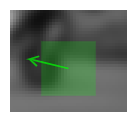
\includegraphics[width=.5\linewidth]{sift-6.png}
          \caption{Orientierung des Merkmals}
          \label{fig:sift6}
        \end{subfigure}%
        \begin{subfigure}{.5\textwidth}
          \centering
          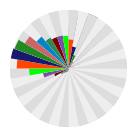
\includegraphics[width=.5\linewidth]{sift-6b.png}
          \caption{Zugehöriges Farbhistogramm (normalisiert)}
          \label{fig:sift6b}
        \end{subfigure}
        \caption{SIFT: Zuordnung der Orientierung}
        \label{fig:sift-orientation}
        \bildquelle{Eigene Darstellung; http://weitz.de/sift/}
    \end{figure}

    \item \textbf{Keypoint descriptor}\newline
    Zuletzt wird nach Anwendung weiterer mathematischer Verfahren eine Art
    Fingerabdruck des Merkmals berechnet (siehe Abbildung \ref{fig:sift7}).
    Dadurch wird die Stabilität gegenüber begrenzter lokaler Formverzerrungen
    und Beleuchtungsänderungen erreicht (siehe Abbildung \ref{fig:sift}).
    \parencite{sift-web-descriptor}

    \begin{figure}[H]
        \centering
        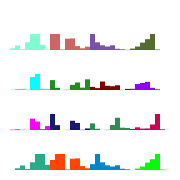
\includegraphics[width=5cm]{sift-7}
        \caption{SIFT: Pro Schlüsselpunkt erzeugte Deskriptoren (Fingerabdruck)}
        \label{fig:sift7}
        \bildquelle{Eigene Darstellung; http://weitz.de/sift/}
    \end{figure}
\end{enumerate}

Nach Anwendung dieses Algorithmus sollte man bei einem 500x500 Pixel großen Bild
mit rund 2000 robusten Merkmalen rechnen. Werden die gefundenen Merkmale in
einer Datenbank gespeichert, können sie in nahezu Echtzeit auf die
Schlüsselpunkte eines Suchbilds verglichen werden.
\parencite{sift-distinctive-features}

Ein ähnlicher, jedoch bis 2033 patentierter\footnote{https://patents.google.com/patent/CN103640018A/en [09.12.2022]}, Algorithmus zur Erkennung von Bildmerkmalen ist der
\glqq{}Speeded up robust features (SURF)\grqq{} \parencite{sift-surf}. Ferner
gibt es viele ähnliche frei verfügbare Algorithmen der Gruppe
\glqq{}Bildmerkmalsfindung\grqq{}.

\begin{figure}[H]
    \centering
    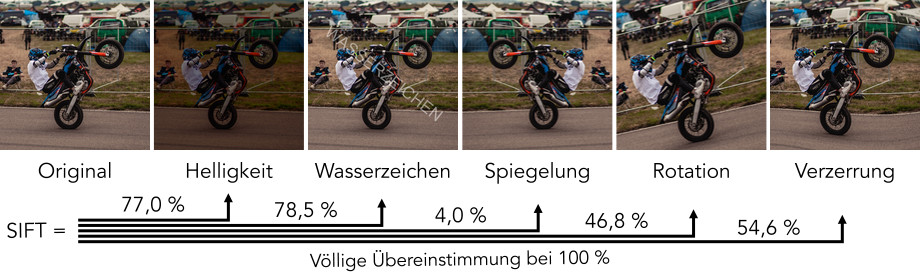
\includegraphics[width=\textwidth]{sift}
    \caption{SIFT: Anwendung an verschiedenen Testbildern}
    \label{fig:sift}
    \bildquelle{Eigene Darstellung}
\end{figure}
